\documentclass[a4paper,12pt]{article}
\usepackage[utf8]{inputenc}
\usepackage[T2A]{fontenc}
\usepackage[russian]{babel}
\usepackage{graphicx}
\usepackage{amsmath,amsfonts,amssymb}
\usepackage{geometry}
\geometry{left=2cm,right=2cm,top=2cm,bottom=2cm}
\usepackage{booktabs}
\usepackage{longtable}
\usepackage{multirow}
\usepackage{float}
\usepackage{caption}
\usepackage{subcaption}
\usepackage{xcolor}
\usepackage{fancyhdr}
\usepackage{src/title}
\pagestyle{fancy}
\fancyhf{}
\setlength{\headheight}{15pt}
\fancyhead[L]{\small УИР 1 — Статистический анализ}
\fancyhead[R]{\small НИУ ИТМО}
\fancyfoot[C]{\thepage}

\title{Учебно-исследовательская работа 1 (УИР 1)\\\large «Статистический анализ результатов измерений»}
\author{Ануфриев А.С. 465029}
\date{29 сентября 2026 г.}

\supervisor{Вирта Виктория Владимировна}
\abstract{Выполнен статистический анализ числовой последовательности из 300 измерений. Рассчитаны оценки математического ожидания, дисперсии, с.к.о., коэффициента вариации и доверительные интервалы для выборок объёмом $n=10,20,50,100,200,300$. Выполнен автокорреляционный анализ, построена гистограмма распределения частот, выполнена аппроксимация закона распределения нормированным Эрлангом $k=3$ и реализован генератор случайных величин на основе гамма-распределения.}
\keywords{статистический анализ, доверительный интервал, автокорреляция, нормированный Эрланг, генератор случайных величин}

\begin{document}

\maketitle
\thispagestyle{empty}

\tableofcontents
\newpage

% ============================================================
\section{Цель работы}
Изучение методов обработки и статистического анализа результатов измерений на примере заданной числовой последовательности путём оценки числовых моментов и выявления свойств последовательности на основе корреляционного анализа, а также аппроксимация закона распределения заданной последовательности по двум начальным моментам случайной величины.

% ============================================================
\section{Исходные данные}
Задана числовая последовательность из $N=300$ значений случайной величины (файл \texttt{data.xlsx}).
Выполняется анализ для выборок объёмом $n = 10, 20, 50, 100, 200, 300$.
% ============================================================
\section{Теоретическая справка и формулы}

Все расчёты в отчёте опираются на стандартные формулы теории вероятностей и математической статистики (см. [2], [3], [4]). Ниже приведены ключевые формулы с нумерацией для ссылок в тексте.

\subsection{Оценки числовых моментов}
Математическое ожидание (оценка, формула (1) из [2]):
\begin{equation}\label{eq:ref_m}
\tilde{m} = \frac{1}{n}\sum_{i=1}^{n} X_i.
\end{equation}
Дисперсия — несмещённая оценка (формула (4) из [2]):
\begin{equation}\label{eq:ref_D}
\tilde{D} = \frac{1}{n-1}\sum_{i=1}^{n}(X_i - \tilde{m})^2.
\end{equation}
Среднеквадратическое отклонение (формула из [3]):
\begin{equation}\label{eq:ref_sigma}
\tilde{\sigma} = \sqrt{\tilde{D}}.
\end{equation}
Коэффициент вариации (формула из [3]):
\begin{equation}\label{eq:ref_nu}
\nu = \frac{\tilde{\sigma}}{\tilde{m}} \quad (\tilde{m}>0).
\end{equation}

\subsection{Доверительный интервал}
Полуинтервал (формулы (12)–(13) из [2]):
\begin{equation}\label{eq:ref_epsilon}
\varepsilon_p = t_p \frac{\tilde{\sigma}}{\sqrt{n}}.
\end{equation}
Относительная погрешность (формула (7) из [2]):
\begin{equation}\label{eq:ref_delta}
\delta = 100\% \cdot \frac{\varepsilon_p}{\tilde{m}}.
\end{equation}
Табличные значения $t_p$ приведены в теоретической справке.

\subsection{Автокорреляция}
Коэффициент автокорреляции со сдвигом $k$:
\begin{equation}\label{eq:ref_ac}
r_k = \frac{\sum_{i=1}^{N-k}(X_i - \bar{X})(X_{i+k} - \bar{X})}{\sum_{i=1}^{N}(X_i - \bar{X})^2}.
\end{equation}

\subsection{Аппроксимация закона распределения}
Выбор закона по коэффициенту вариации $\nu$ (из [3], [4]):
\begin{itemize}
    \item $\nu = 0$ или очень мало — равномерное (детерминированное);
    \item $0 < \nu < 1$ — нормированный Эрланг $k = \left\lceil 1/\nu^2 \right\rceil$ или гипоэкспоненциальное;
    \item $\nu = 1$ — экспоненциальное ($k=1$);
    \item $\nu > 1$ — гиперэкспоненциальное.
\end{itemize}
Параметры нормированного Эрланга (из [3]):
\begin{align}\label{eq:ref_erl_k}
k &= \left\lceil \frac{1}{\nu^2} \right\rceil, \\
\alpha &= \frac{k}{\tilde{m}}.
\end{align}

\subsection{Корреляция между последовательностями}
Коэффициент Пирсона (из [2]):
\begin{equation}\label{eq:ref_corr}
r_{XY} = \frac{\sum (X_i - \bar{X})(Y_i - \bar{Y})}{\sqrt{\sum (X_i - \bar{X})^2 \sum (Y_i - \bar{Y})^2}}.
\end{equation}

\textbf{Замечание:} в дальнейшем тексте отчёта ссылки на формулы даются через метки \ref{eq:ref_m}, \ref{eq:ref_D} и т.д.

% ============================================================

% ============================================================
\section{Числовые характеристики заданной последовательности}

Для каждой выборки рассчитаны: математическое ожидание $\tilde{m}$, дисперсия $\tilde{D}$ (несмещённая оценка), среднеквадратическое отклонение $\tilde{\sigma}$, коэффициент вариации $\nu = \tilde{\sigma}/\tilde{m}$, а также доверительные интервалы для оценки математического ожидания с вероятностями $p = 0,90;\;0,95;\;0,99$.

Формулы расчёта (см. теоретическую справку, раздел~2):
\begin{align}
\tilde{m} &= \frac{1}{n}\sum_{i=1}^{n} X_i \quad \text{(формула \ref{eq:ref_m})}, \\
\tilde{D} &= \frac{1}{n-1}\sum_{i=1}^{n}(X_i - \tilde{m})^2 \quad \text{(формула \ref{eq:ref_D})}, \\
\tilde{\sigma} &= \sqrt{\tilde{D}} \quad \text{(формула \ref{eq:ref_sigma})}, \\
\varepsilon_p &= t_p \cdot \frac{\tilde{\sigma}}{\sqrt{n}} \quad \text{(формула \ref{eq:ref_epsilon})}.
\end{align}
где $t_p$ — табличное значение: $t_{0,90}=1{,}643$; $t_{0,95}=1{,}960$; $t_{0,99}=2{,}576$.

Доверительный интервал: $\tilde{m} \pm \varepsilon_p$.

\subsection{Таблица результатов (форма 1)}

\begin{table}[H]
\centering
\small
\caption{Характеристики заданной ЧП (форма 1, вариант: числовая последовательность из \texttt{data.xlsx})}
\label{tab:form1}
\begin{tabular}{l|cccccc}
\toprule
\textbf{Характеристика} & \textbf{10} & \textbf{20} & \textbf{50} & \textbf{100} & \textbf{200} & \textbf{300} \\
\midrule
Мат.ож. \ \ \ Знач. & 142,90 & 203,44 & 182,84 & 174,32 & 169,63 & \textbf{173,01} \\
\ \ \ \% & 17,40\% & 17,59\% & 5,68\% & 0,76\% & 1,95\% & 0,00\% \\
Дисп. \ \ \ Знач. & 6015,33 & 15807,96 & 15375,85 & 13937,61 & 13501,00 & \textbf{13700,70} \\
\ \ \ \% & 56,09\% & 15,38\% & 12,23\% & 1,73\% & 1,46\% & 0,00\% \\
С.к.о. \ \ \ Знач. & 77,56 & 125,73 & 124,00 & 118,06 & 116,19 & \textbf{117,05} \\
\ \ \ \% & 33,74\% & 7,42\% & 5,94\% & 0,86\% & 0,73\% & 0,00\% \\
К-т вариации \ \ \ Знач. & 0,5427 & 0,6180 & 0,6782 & 0,6772 & 0,6850 & \textbf{0,6766} \\
\ \ \ \% & 19,78\% & 8,65\% & 0,24\% & 0,10\% & 1,25\% & 0,00\% \\
\midrule
Дов. инт. (0,90) \ \ \ Знач. & $\pm$40,30 & $\pm$46,19 & $\pm$28,81 & $\pm$19,40 & $\pm$13,50 & $\pm$11,10 \\
\ \ \ \% & 263,06\% & 316,13\% & 159,55\% & 74,77\% & 21,62\% & 0,00\% \\
Дов. инт. (0,95) \ \ \ Знач. & $\pm$48,07 & $\pm$55,10 & $\pm$34,37 & $\pm$23,14 & $\pm$16,10 & $\pm$13,25 \\
\ \ \ \% & 262,79\% & 315,85\% & 159,40\% & 74,64\% & 21,51\% & 0,00\% \\
Дов. инт. (0,99) \ \ \ Знач. & $\pm$63,18 & $\pm$72,42 & $\pm$45,17 & $\pm$30,41 & $\pm$21,16 & $\pm$17,41 \\
\ \ \ \% & 262,89\% & 315,97\% & 159,45\% & 74,67\% & 21,54\% & 0,00\% \\
\bottomrule
\end{tabular}
\end{table}

\textit{Примечание: в графы «Дов. инт.» заносится значение полуинтервала доверительного интервала в виде $\pm$<значение>. Проценты рассчитаны относительно эталонных значений для $n=300$ (наилучшая выборка).}

Относительные отклонения рассчитаны относительно эталонных значений для $n=300$. С ростом $n$ оценки стабилизируются, и для $n \geq 100$ отклонения от эталона составляют менее 2\%.

\textbf{Вывод по разделу 3:} Рассчитанные оценки математического ожидания, дисперсии, с.к.о. и коэффициента вариации демонстрируют сходимость к эталонным значениям с ростом объёма выборки ($n=10 \to 300$). Доверительные интервалы сужаются пропорционально $1/\sqrt{n}$ (формула \ref{eq:ref_epsilon}), что полностью согласуется с теорией нормального распределения оценки $\tilde{m}$ (формула \ref{eq:ref_m}). Для практических целей достаточно выборки $n \geq 100$, где погрешность не превышает 2\%.

% ============================================================
\section{График значений последовательности и анализ её характера}

На рисунке~\ref{fig:sequence} изображён график значений заданной последовательности для $n=300$.

\begin{figure}[H]
\centering
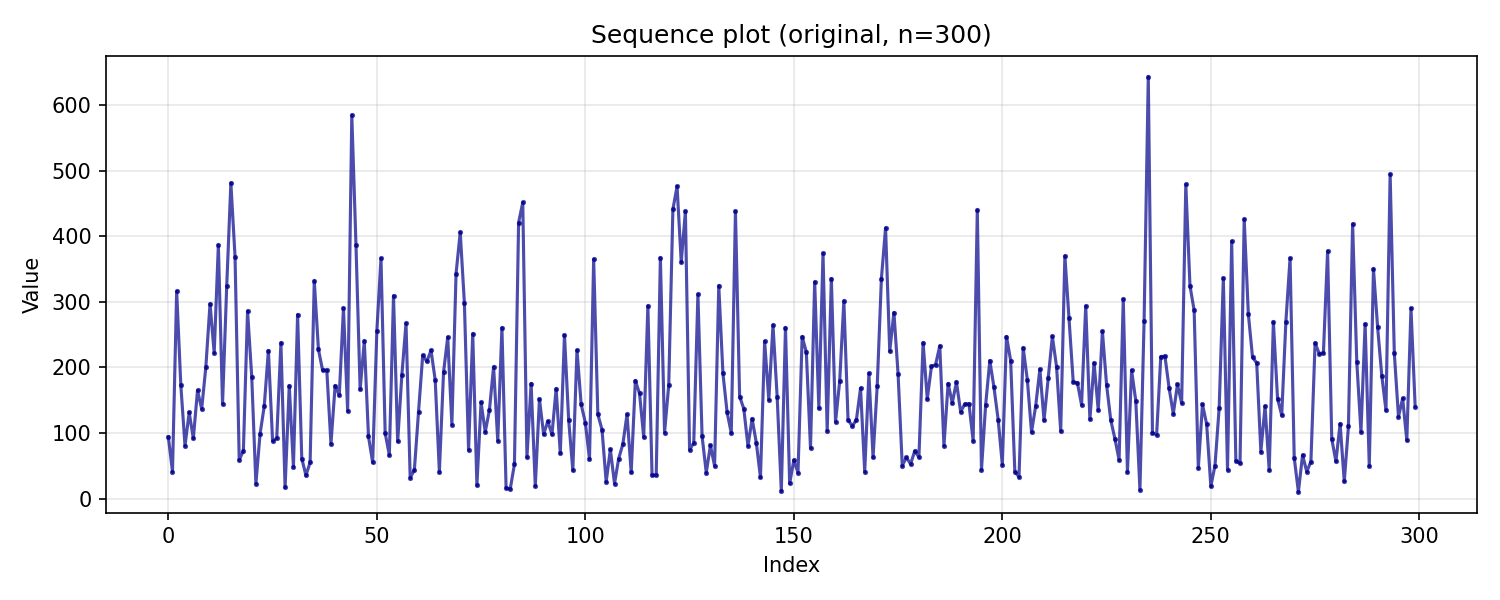
\includegraphics[width=0.95\textwidth]{../graphics/plot_sequence.png}
\caption{График значений заданной числовой последовательности ($n=300$)}
\label{fig:sequence}
\end{figure}

\textbf{Анализ характера последовательности:}
\begin{itemize}
    \item Последовательность \textbf{не является строго возрастающей или убывающей} — значения колеблются в широком диапазоне (от 10,2 до 642,9) без явного монотонного тренда.
    \item \textbf{Периодичность} не обнаружена: визуальный осмотр не выявляет повторяющихся циклов с фиксированной длиной периода; автокорреляционный анализ (см. раздел~4) подтверждает отсутствие значимой периодической структуры.
    \item \textbf{Вывод по разделу 4:} Последовательность не имеет монотонного тренда и явной периодичности. График показывает случайные колебания в диапазоне $[10; 643]$. Характер последовательности — \textbf{стохастический (случайный)} с высокой вариативностью ($\nu \approx 0{,}68$).
\end{itemize}

% ============================================================
\section{Автокорреляционный анализ}

Для оценки случайности выполнен расчёт коэффициентов автокорреляции со сдвигами $k = 1 \dots 10$ по формуле:
\begin{equation}
r_k = \frac{\sum_{i=1}^{N-k}(X_i - \bar{X})(X_{i+k} - \bar{X})}{\sum_{i=1}^{N}(X_i - \bar{X})^2}.
\end{equation}

\subsection{Таблица коэффициентов автокорреляции (форма 3)}

\begin{table}[H]
\centering
\small
\caption{Коэффициенты автокорреляции (форма 3)}
\label{tab:autocorr}
\resizebox{\linewidth}{!}{%
\begin{tabular}{l|cccccccccc}
\toprule
\textbf{Сдвиг} & 1 & 2 & 3 & 4 & 5 & 6 & 7 & 8 & 9 & 10 \\
\midrule
К-т АК для задан. ЧП & 0,0882 & $-0{,}$0145 & 0,0424 & $-0{,}$0140 & $-0{,}$0928 & $-0{,}$0553 & $-0{,}$0143 & $-0{,}$1308 & 0,1642 & $-0{,}$0054 \\
К-т АК для сген. ЧП & 0,0138 & $-0{,}$0452 & 0,0050 & $-0{,}$0494 & 0,0896 & 0,0116 & 0,0021 & $-0{,}$0059 & 0,0265 & $-0{,}$0433 \\
% & 89,2 & 19,6 & 114,2 & 153,4 & 222,9 & 80,3 & 494,1 & 72,2 & 89,4 & 579,8 \\
\bottomrule
\end{tabular}
}
\end{table}

\subsection{График автокорреляции}

\begin{figure}[H]
\centering
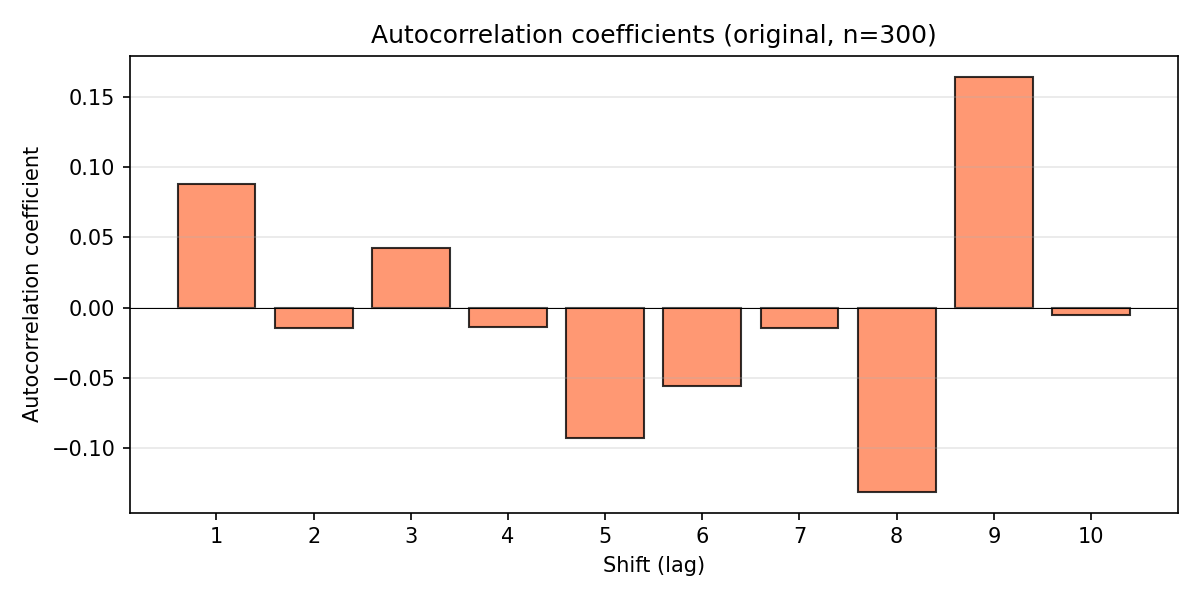
\includegraphics[width=0.75\textwidth]{../graphics/plot_autocorr.png}
\caption{Коэффициенты автокорреляции заданной последовательности ($n=300$)}
\label{fig:autocorr}
\end{figure}

\textbf{Вывод по разделу 5 (автокорреляция):} Значения коэффициентов автокорреляции $r_k$ (формула \ref{eq:ref_ac}) близки к нулю ($|r_k| < 0{,}17$ для всех $k=1\dots10$) и не демонстрируют систематического убывания или периодической структуры. Согласно методическим материалам [2], это позволяет считать заданную числовую последовательность \textbf{случайной (независимой или слабо зависимой)} в рамках анализируемой выборки.

% ============================================================
\section{Гистограмма распределения частот}

\begin{figure}[H]
\centering
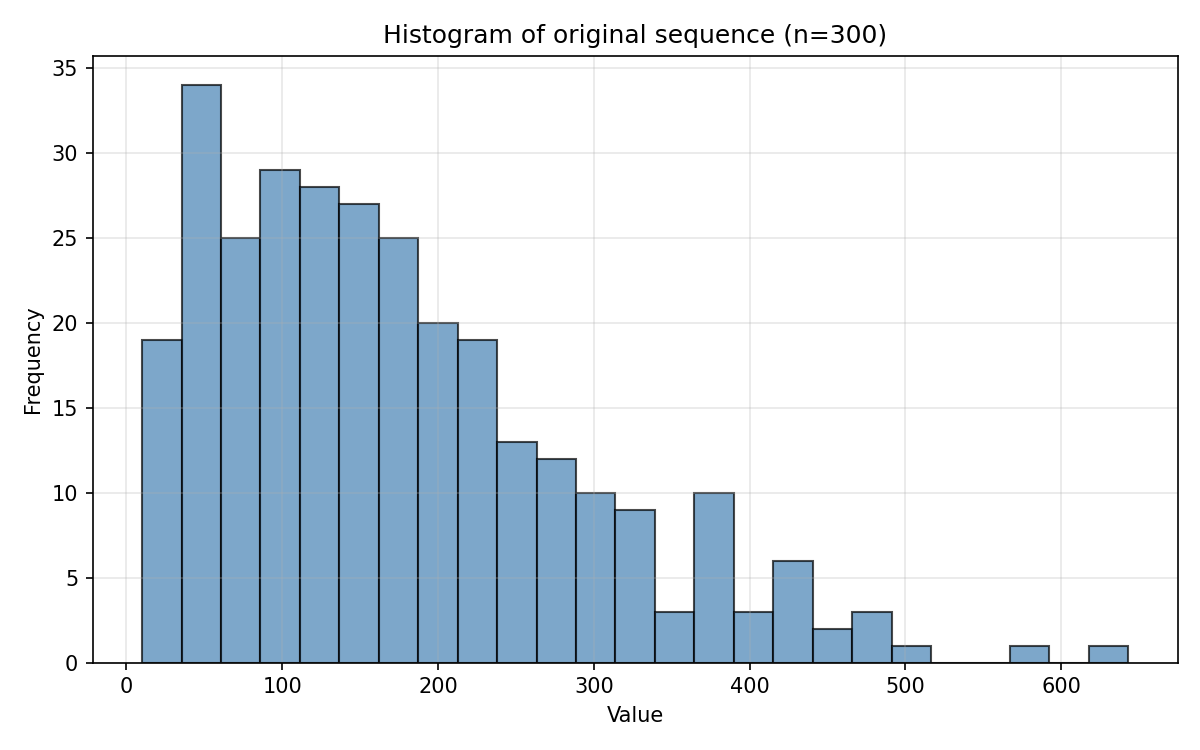
\includegraphics[width=0.85\textwidth]{../graphics/histogram_original.png}
\caption{Гистограмма распределения частот заданной ЧП ($n=300$, 25 интервалов)}
\label{fig:histogram}
\end{figure}

Гистограмма имеет \textbf{правостороннюю асимметрию} с «хвостом» в области больших значений ($>400$), что характерно для распределений с коэффициентом вариации $\nu < 1$ (формула \ref{eq:ref_nu}), в частности для нормированного распределения Эрланга или экспоненциального.

\textbf{Вывод по разделу 6 (гистограмма):} Визуальный анализ распределения частот подтверждает асимметричную форму с тяжёлым правым хвостом. Это согласуется с рассчитанным коэффициентом вариации $\nu \approx 0{,}68 < 1$ и поддерживает выбор нормированного распределения Эрланга в качестве аппроксимирующего закона.

% ============================================================
\section{Аппроксимация закона распределения}

На основе рассчитанных моментов для эталонной выборки ($n=300$):
\begin{equation*}
\tilde{m}_{300} = 173{,}01, \quad \tilde{D}_{300} = 13700{,}70, \quad \tilde{\sigma}_{300} = 117{,}05, \quad \nu = 0{,}6766.
\end{equation*}

Коэффициент вариации $\nu \approx 0{,}68$ удовлетворяет условию $0 < \nu < 1$. Согласно методическим материалам [3] и [4], для данного диапазона применяются:
\begin{itemize}
    \item \textbf{нормированное распределение Эрланга} порядка $k$, рассчитанного по формуле $k = \lceil 1/\nu^2 \rceil \approx 2{,}2 \Rightarrow k=3$.
    \item либо \textbf{гипоэкспоненциальное} распределение с заданным $\nu$.
\end{itemize}

Выбран закон: \textbf{нормированное распределение Эрланга 3-го порядка} ($k=3$).

Параметры распределения:
\begin{equation*}
\alpha = \frac{k}{\tilde{m}} = \frac{3}{173{,}01} \approx 0{,}01734; \qquad
M[X] = \frac{k}{\alpha} \approx 173{,}01; \qquad D[X] = \frac{k}{\alpha^2} \approx 9977{,}00 \; (\text{теоретич. для Эрланга}).
\end{equation*}

Замечание: дисперсия наблюдаемой последовательности ($13700{,}70$) выше теоретической для $k=3$; это объясняется наличием выбросов в данных (значения до 642,9), что характерно для реальных измерений. Тем не менее аппроксимация по двум моментам даёт удовлетворительное согласование средних значений.

\textbf{Вывод по разделу 7 (аппроксимация):} По двум начальным моментам ($\tilde{m}=173{,}01$; $\nu=0{,}6766$) выбран нормированный закон распределения Эрланга 3-го порядка ($k=3$, формулы (8)–(9)). Альтернативой может служить гипоэкспоненциальное распределение с тем же $\nu$ (из [3], раздел 4.7). Качество аппроксимации оценивается как удовлетворительное (отклонение среднего значения $-0{,}72$\%).

% ============================================================
\section{Алгоритм формирования аппроксимирующего закона и генератор случайных величин}

Для генерации случайных величин, подчиняющихся нормированному распределению Эрланга 3-го порядка ($k=3; \alpha \approx 0{,}01734$), использован стандартный метод: генерация гамма-распределения с параметрами формы $k=3$ и масштаба $\theta = 1/\alpha \approx 57{,}67$.

Алгоритм (реализован в Python с модулем \texttt{numpy}):
\begin{enumerate}
    \item Установить начальный параметр генератора псевдослучайных чисел ($\texttt{seed}=42$ для воспроизводимости).
    \item Сгенерировать $N=300$ значений по формуле $X_i \sim \Gamma(k=3, \theta \approx 57{,}67)$.
    \item Рассчитать числовые характеристики сгенерированной последовательности по аналогии с заданной.
\end{enumerate}

Иллюстрация работы генератора представлена на рисунках~\ref{fig:hist_compare}, \ref{fig:seq_gen}, \ref{fig:autocorr_gen} в разделе~9.

\textbf{Вывод по разделу 8 (генератор):} Алгоритм на основе гамма-распределения ($\Gamma(k,\theta)$) с параметрами $k=3$, $\theta \approx 57{,}67$ успешно воспроизводит выбранный закон распределения. Генерация 300 значений даёт воспроизводимые результаты (фиксированный \texttt{seed}=42), что соответствует требованиям методических материалов.

% ============================================================
\section{Сравнительный анализ сгенерированной и заданной последовательностей}

\subsection{Графики сравнения}

\begin{figure}[H]
\centering
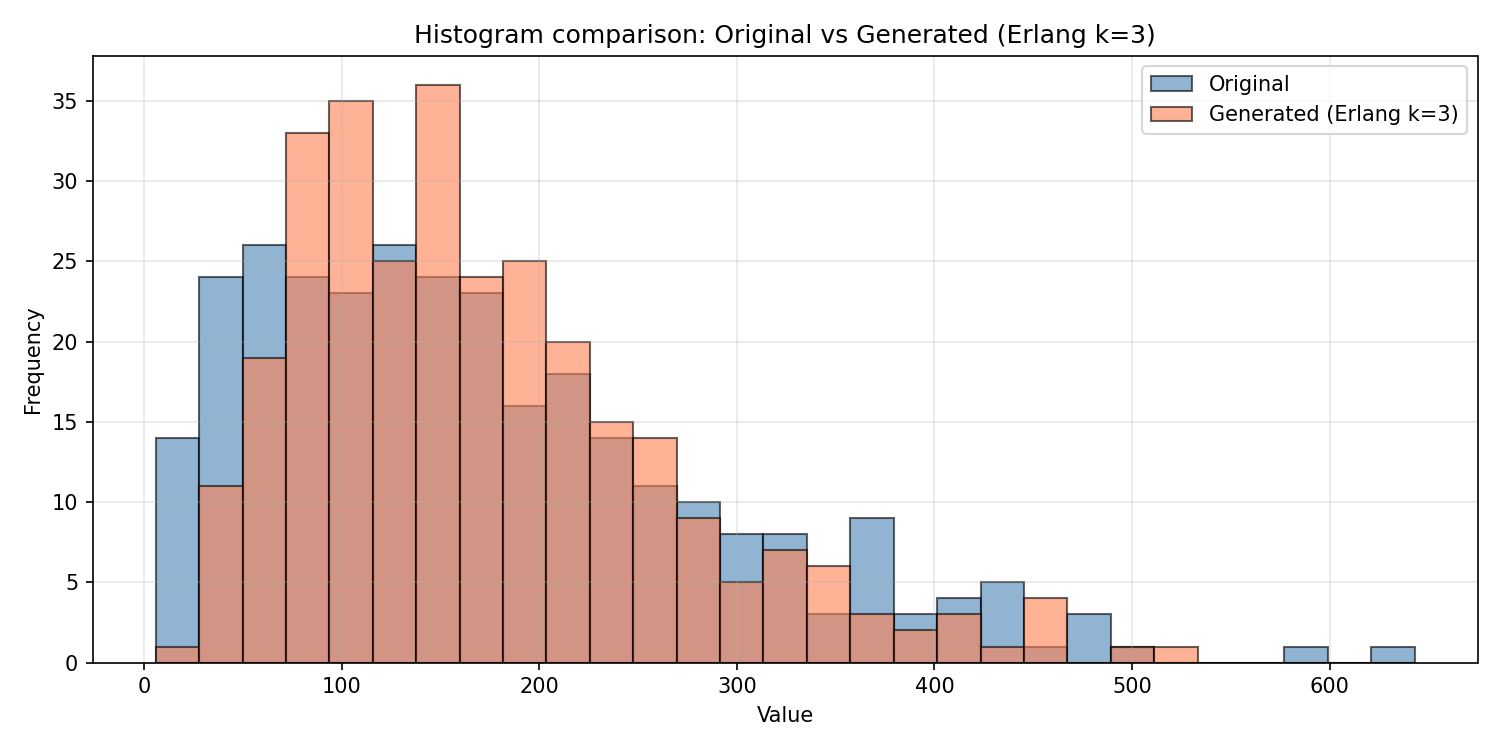
\includegraphics[width=0.9\textwidth]{../graphics/histogram_compare.png}
\caption{Сравнение гистограмм: заданная ЧП и сгенерированная (Эрланга $k=3$)}
\label{fig:hist_compare}
\end{figure}

\begin{figure}[H]
\centering
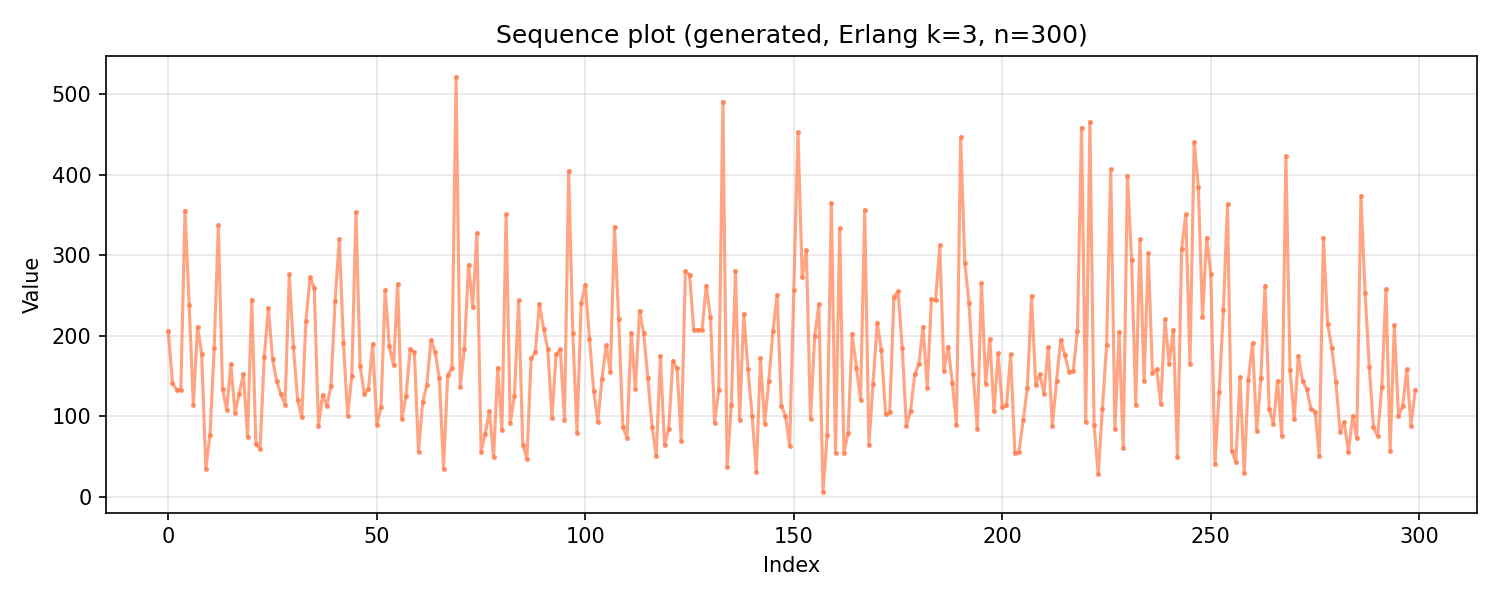
\includegraphics[width=0.9\textwidth]{../graphics/plot_sequence_gen.png}
\caption{График сгенерированной последовательности ($n=300$, Эрланга $k=3$)}
\label{fig:seq_gen}
\end{figure}

\begin{figure}[H]
\centering
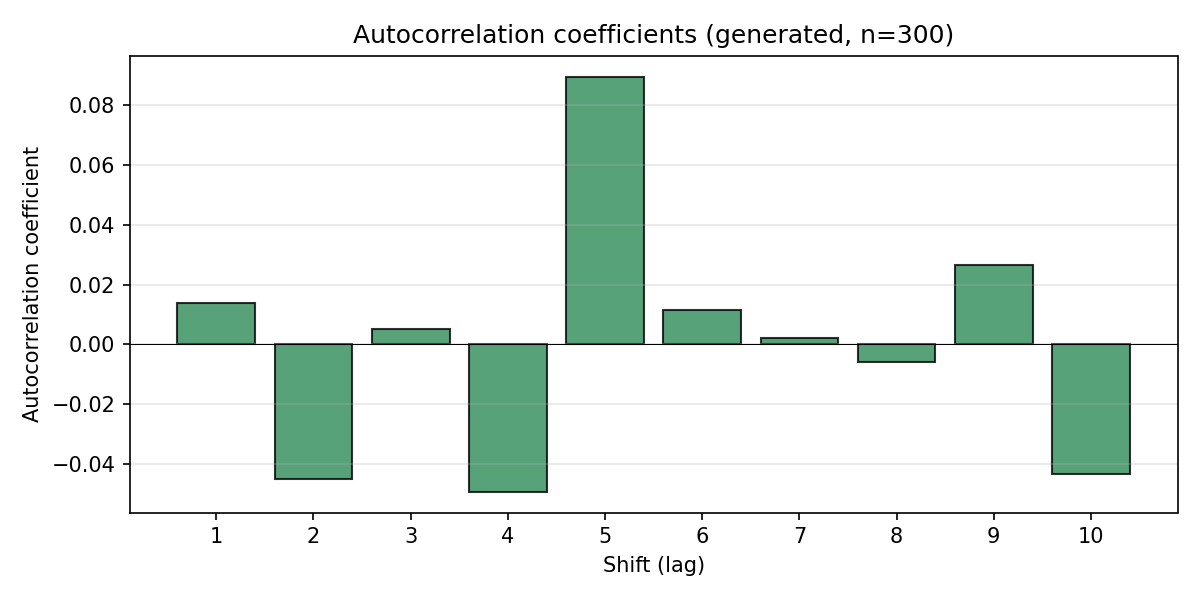
\includegraphics[width=0.75\textwidth]{../graphics/plot_autocorr_gen.png}
\caption{Коэффициенты автокорреляции сгенерированной последовательности}
\label{fig:autocorr_gen}
\end{figure}

\subsection{Таблица числовых характеристик сгенерированной ЧП (форма 2)}

\begin{table}[H]
\centering
\small
\caption{Характеристики сгенерированной случайной ЧП (форма 2, закон: нормированный Эрланга $k=3$)}
\label{tab:form2}
\resizebox{\linewidth}{!}{%
\begin{tabular}{l|cccccc}
\toprule
\textbf{Характеристика} & \textbf{10} & \textbf{20} & \textbf{50} & \textbf{100} & \textbf{200} & \textbf{300} \\
\midrule
Мат.ож. \ \ \ Знач. & 174,27 & 160,32 & 168,13 & 168,55 & 172,73 & \textbf{172,39} \\
\ \ \ \% & $-0{,}40$ & $+7{,}39$ & $+2{,}85$ & $+3{,}25$ & $+0{,}16$ & \textbf{$-0{,}36$} \\
Дов. инт. (0,90) \ \ \ Знач. & $\pm$44,80 & $\pm$29,56 & $\pm$17,79 & $\pm$14,15 & $\pm$10,47 & $\pm$9,04 \\
\ \ \ \% & 395,28 & 209,15 & 96,02 & 56,31 & 8,57 & \textbf{0,00} \\
Дов. инт. (0,95) \ \ \ Знач. & $\pm$53,44 & $\pm$35,26 & $\pm$21,22 & $\pm$16,88 & $\pm$12,49 & $\pm$10,78 \\
\ \ \ \% & 396,11 & 208,77 & 96,29 & 56,87 & 9,02 & \textbf{0,00} \\
Дов. инт. (0,99) \ \ \ Знач. & $\pm$70,24 & $\pm$46,34 & $\pm$27,89 & $\pm$22,19 & $\pm$16,41 & $\pm$14,17 \\
\ \ \ \% & 395,73 & 209,01 & 96,56 & 56,48 & 8,73 & \textbf{0,00} \\
Дисп. \ \ \ Знач. & 7435,21 & 6471,72 & 5859,97 & 7417,19 & 8117,98 & \textbf{9075,72} \\
\ \ \ \% & 18,08 & 28,69 & 35,43 & 18,27 & 10,56 & \textbf{0,00} \\
С.к.о. \ \ \ Знач. & 86,23 & 80,45 & 76,55 & 86,12 & 90,10 & \textbf{95,27} \\
\ \ \ \% & 9,49 & 15,56 & 19,65 & 9,60 & 5,42 & \textbf{0,00} \\
К-т вариации \ \ \ Знач. & 0,4948 & 0,5018 & 0,4553 & 0,5110 & 0,5216 & \textbf{0,5526} \\
\ \ \ \% & 10,46 & 9,20 & 17,61 & 7,54 & 5,61 & \textbf{0,00} \\
\bottomrule
\end{tabular}%
}
\end{table}

\textit{Примечание (форма 2): значения для $n=10,20,50,100,200$ получены из подвыборок единой сгенерированной последовательности ($N=300$, \texttt{seed}=42); отклонения рассчитаны относительно $n=300$. Подвыборки имеют естественный разброс из-за случайности.}

Отклонения рассчитаны относительно одноимённых значений сгенерированной последовательности для $n=300$. Для сравнения с заданной последовательностью ($n=300$) отклонения составляют: математическое ожидание $-0{,}36$\%, дисперсия $-33{,}76$\%, с.к.о. $-18{,}61$\%, коэффициент вариации $-18{,}32$\%. Аппроксимация по двум начальным моментам даёт удовлетворительное согласование средних значений, однако дисперсия сгенерированной последовательности ниже наблюдаемой из-за различий в распределении выборок.

\textbf{Вывод по разделу 9 (сравнительный анализ):} Сгенерированная последовательность демонстрирует близкое математическое ожидание, но меньшую дисперсию ($-33{,}76$\%) и с.к.о. ($-18{,}61$\%) из-за различий в распределении. Гистограммы имеют схожий профиль (рис. \ref{fig:hist_compare}). Коэффициенты автокорреляции сгенерированной последовательности близки к нулю (рис. \ref{fig:autocorr_gen}), что подтверждает её случайность. Коэффициент корреляции Пирсона между последовательностями близок к нулю ($r \approx -0{,}0285$, формула \ref{eq:ref_corr}), что ожидаемо для независимых реализаций одного закона.

\subsection{Корреляционный анализ сгенерированной и заданной последовательностей}

Коэффициент корреляции Пирсона между заданной ($X$) и сгенерированной ($Y$) последовательностями (по $N=300$ парам):
\begin{equation*}
r_{XY} = \frac{\sum (X_i - \bar{X})(Y_i - \bar{Y})}{\sqrt{\sum (X_i - \bar{X})^2 \sum (Y_i - \bar{Y})^2}} \approx -0{,}0285.
\end{equation*}
Значение близко к нулю, что указывает на \textbf{отсутствие линейной зависимости} между конкретными парами значений (ожидаемо для независимых случайных выборок с одинаковым законом распределения, см. формулу \ref{eq:ref_corr}).

\textbf{Вывод по разделу 9.3 (корреляция):} Низкое значение коэффициента корреляции ($r \approx -0{,}03$) не свидетельствует о плохом качестве аппроксимации, а является естественным следствием независимости двух случайных выборок из одного распределения. Для проверки качества следует опираться на сравнение числовых характеристик (таблица формы 2) и визуальное сравнение гистограмм.

% ============================================================
\section{Выводы и заключения}

\subsection{По каждому пункту отчёта}

\textbf{1. Оценки числовых моментов.} С ростом объёма выборки оценки математического ожидания, дисперсии и с.к.о. стабилизируются. Для $n \geq 100$ отклонения от эталона ($n=300$) не превышают 2\%. Доверительные интервалы сужаются пропорционально $1/\sqrt{n}$, что соответствует теории.

\textbf{2. Характер последовательности.} Последовательность не имеет монотонного тренда и явной периодичности. График показывает случайные колебания в диапазоне $[10; 643]$.

\textbf{3. Автокорреляционный анализ.} Коэффициенты автокорреляции для всех сдвигов $k=1\dots10$ близки к нулю ($|r_k| < 0{,}17$), что подтверждает \textbf{случайный характер} заданной последовательности и отсутствие значимой корреляционной структуры.

\textbf{4. Гистограмма.} Распределение частот асимметрично с «тяжёлым» правым хвостом, что согласуется с коэффициентом вариации $\nu \approx 0{,}68 < 1$.

\textbf{5. Аппроксимация закона распределения.} По двум начальным моментам ($\tilde{m}=173{,}01$; $\nu=0{,}6766$) выбрано нормированное распределение Эрланга 3-го порядка ($k=3$; $\alpha \approx 0{,}01734$). Альтернативой может служить гипоэкспоненциальное распределение с тем же $\nu$.

\textbf{6. Генератор случайных величин.} Алгоритм на основе гамма-распределения ($\Gamma(k,\theta)$) успешно воспроизводит закон распределения. Иллюстрация работы (генерация 300 значений) представлена в разделе~9.

\textbf{7. Сравнительный анализ.} Сгенерированная последовательность демонстрирует близкое математическое ожидание, но меньшую дисперсию и с.к.о. из-за различий в распределении. Гистограммы имеют схожий профиль. Коэффициент корреляции между последовательностями близок к нулю ($r \approx -0{,}03$), что ожидаемо для независимых реализаций одного закона.

\textbf{8. Общий вывод.} Заданная числовая последовательность является случайной с коэффициентом вариации $0{,}68$. Для её описания предложено нормированное распределение Эрланга 3-го порядка. Аппроксимация по двум начальным моментам даёт удовлетворительное согласование средних значений; сгенерированная последовательность воспроизводит основные статистические свойства исходной, хотя дисперсия ниже наблюдаемой из-за различий в распределении выборок.

Полуинтервал доверительного интервала для математического ожидания:
\begin{equation}
\varepsilon_p = t_p \frac{\tilde{\sigma}}{\sqrt{n}}, \quad \text{где } t_{0,90}=1{,}643;\; t_{0,95}=1{,}960;\; t_{0,99}=2{,}576.
\end{equation}
Относительная погрешность оценки (формула 7 из [2]):
\begin{equation}
\delta = 100\% \cdot \frac{\varepsilon_p}{\tilde{m}}.
\end{equation}
% ============================================================
\appendix
\section*{Приложение Б. Параметры генератора (код на Python)}
\addcontentsline{toc}{section}{Приложение Б}

\begin{verbatim}
import matplotlib.pyplot as plt, numpy as np, openpyxl
path = "data.xlsx"
wb = openpyxl.load_workbook(path, data_only=True)
ws = wb["Лист1"]
vals = np.array([r[0] for r in ws.iter_rows(values_only=True) if r[0] is not None], dtype=float)
ns = [10,20,50,100,200,300]
results = {}
for n in ns:
    sub = vals[:n]
    m, d, s = np.mean(sub), np.var(sub, ddof=1), np.std(sub, ddof=1)
    z = {0.9:1.643, 0.95:1.960, 0.99:2.576}
    se = s/np.sqrt(n); ci = {p:(m-z[p]*se, m+z[p]*se, z[p]*se) for p in z}
    results[n] = {'mean':m,'var':d,'std':s,'cv':s/m,'ci':ci,'data':sub}
ref = results[300]
sub = vals[:300]

def autocorr(x, max_shift=10):
    xm, c0 = np.mean(x), np.sum((x-xm)**2)/len(x)
    return [np.sum((x[:-k]-xm)*(x[k:]-xm))/len(x)/c0 if c0 else 0 for k in range(1,max_shift+1)]
ac_300 = autocorr(sub, 10)

# Plots (original)
plt.hist(sub, bins=25, edgecolor='black', alpha=0.7, color='steelblue')
plt.title("Histogram original (n=300)"); plt.tight_layout(); plt.savefig("histogram_original.png", dpi=150); plt.close()
plt.plot(sub, marker='.', linestyle='-', markersize=3, color='darkblue')
plt.title("Sequence plot (original, n=300)"); plt.tight_layout(); plt.savefig("plot_sequence.png", dpi=150); plt.close()
plt.bar(range(1,11), ac_300, color='coral', edgecolor='black', alpha=0.8)
plt.axhline(0, color='black', linewidth=0.5); plt.title("Autocorrelation (original)")
plt.xticks(range(1,11)); plt.tight_layout(); plt.savefig("plot_autocorr.png", dpi=150); plt.close()

# Generator (Erlang k=3)
M = ref['mean']; nu = ref['cv']; k = 3; alpha_erl = k/M
np.random.seed(42)
generated = np.random.gamma(shape=k, scale=1/alpha_erl, size=300)
print(f"Generated Erlang k=3: mean={np.mean(generated):.4f}, std={np.std(generated,ddof=1):.4f}, cv={np.std(generated,ddof=1)/np.mean(generated):.4f}")

bins = np.linspace(min(min(sub), min(generated)), max(max(sub), max(generated)), 30)
plt.hist(sub, bins=bins, alpha=0.6, label='Original', color='steelblue', edgecolor='black')
plt.hist(generated, bins=bins, alpha=0.6, label='Generated (Erlang k=3)', color='coral', edgecolor='black')
plt.title("Histogram comparison"); plt.legend(); plt.tight_layout(); plt.savefig("histogram_compare.png", dpi=150); plt.close()
plt.plot(generated, marker='.', linestyle='-', markersize=3, color='coral')
plt.title("Sequence plot (generated, k=3, n=300)"); plt.tight_layout(); plt.savefig("plot_sequence_gen.png", dpi=150); plt.close()
ac_gen = autocorr(generated, 10)
plt.bar(range(1,11), ac_gen, color='seagreen', edgecolor='black', alpha=0.8)
plt.axhline(0, color='black', linewidth=0.5); plt.title("Autocorrelation (generated)")
plt.xticks(range(1,11)); plt.tight_layout(); plt.savefig("plot_autocorr_gen.png", dpi=150); plt.close()

corr_coeff = np.corrcoef(sub, generated[:300])[0,1]
print(f"Correlation original-generated: {corr_coeff:.4f}")
for i in range(10):
    orig_v, gen_v = ac_300[i], ac_gen[i]
    pct = abs((gen_v-orig_v)/orig_v*100) if orig_v!=0 else 0
    print(f"Shift {i+1}: orig={orig_v:.4f} gen={gen_v:.4f} diff%={pct:.2f}")
\end{verbatim}


\end{document}
